\documentclass[letterpaper]{aastex61}

% to-do list
% ----------
% - add items here
% style notes
% -----------
% - This file generates by Makefile; don't be typing ``pdflatex'' or some bullshit.
% - Line break between sentences to make the git diffs readable.
% - Use \, as a multiply operator.
% - Reserve () for function arguments; use [] or {} for outer shit.
% - Use \sectionname not Section, \figname not Figure, \documentname not Article or Paper or paper.

% packages
\definecolor{cbblue}{HTML}{3182bd}
\usepackage{microtype}  % ALWAYS!
\usepackage{amsmath,amssymb}
\usepackage{tikz}
\hypersetup{backref,breaklinks,colorlinks,urlcolor=cbblue,linkcolor=cbblue,citecolor=black}
\graphicspath{{.}{figures/}}

% define macros for text
\newcommand{\project}[1]{\textsl{#1}}
\newcommand{\acronym}[1]{{\small{#1}}}
\newcommand{\gaia}{\project{Gaia}}
\newcommand{\rave}{\project{\acronym{RAVE}}}
\newcommand{\apogee}{\project{\acronym{APOGEE}}}
\newcommand{\tmass}{\project{\acronym{2MASS}}}
\newcommand{\documentname}{Article}
\newcommand{\sectionname}{Section}
\newcommand{\figname}{Figure}
\newcommand{\eqname}{Equation}
\newcommand{\dr}{\acronym{DR1}}
\newcommand{\tgas}{\acronym{TGAS}}
\newcommand{\etal}{\textit{et al}.}

\newcommand{\objname}{moving group}

% define macros for math
\newcommand{\given}{\,|\,}
\newcommand{\normal}{{\mathcal{N}}}
\newcommand{\dd}{\mathrm{d}}
\newcommand{\transp}[1]{{#1}^{\!\mathsf{T}}}
\newcommand{\inv}[1]{{#1}^{-1}}
\newcommand{\bs}[1]{\boldsymbol{#1}}
\newcommand{\vperp}{\bs{v}^\perp}
\newcommand{\propm}{\bs{\mu}}
\newcommand{\mat}[1]{\mathbf{#1}}
\renewcommand{\vec}[1]{\bs{#1}}
\newcommand{\kms}{\ensuremath{\rm km~s^{-1}}}
\newcommand{\msun}{{\rm M}_\odot}
\newcommand{\data}{\mathrm{data}}
\newcommand{\snr}{[S/N]_\varpi}
\newcommand{\eye}{\mathbb{I}}
\newcommand{\absdvtan}{\ensuremath{|\Delta\vec v_\mathrm{t}|}}
\newcommand{\estimates}{\ensuremath{\{\hat{\varpi_i},\hat{\mu_{\alpha,i}},\hat{\mu_{\delta,i}},\hat{v_{r,i}}\}}}

\newcommand{\todo}[1]{{\color{blue}TODO:#1}}

\begin{document}\sloppy\sloppypar\raggedbottom\frenchspacing % trust me

\title{A New? Nearby Young Moving Group -- Latyshev-2 rediscovered?}

\author{Semyeong Oh\altaffilmark{\pu,\lead} \etal}

% Affiliations
\newcommand{\pu}{1}
\newcommand{\lead}{2}
\newcommand{\ccpp}{3}
\newcommand{\mpia}{4}
\newcommand{\cca}{5}

\altaffiltext{\pu}{Department of Astrophysical Sciences,
                   Princeton University, Princeton, NJ 08544, USA}
\altaffiltext{\lead}{To whom correspondence should be addressed:
                     \texttt{semyeong@astro.princeton.edu}}
\altaffiltext{\ccpp}{Center for Cosmology and Particle Physics,
                     Department of Physics,
                     New York University, 4 Washington Place,
                     New York, NY 10003, USA}
\altaffiltext{\mpia}{Max-Planck-Institut f\"ur Astronomie,
                     K\"onigstuhl 17, D-69117 Heidelberg, Germany}
\altaffiltext{\cca}{Center for Computational Astrophysics, 162 5th Ave, New York, NY 10003, USA}


\begin{abstract}
  We report the discovery of a new, nearby \objname\ composed of XX stars
  in the \gaia\ DR 1 at Galactic coordinates $(l, b, d) = ()$.
  Notable members include XXX.
  The system is discovered as an aggregate of connected co-moving pairs in our recent study.
  Many of the member stars show signs of youth such as X-ray emission or infrared excess.
  We obtain low resolution spectra of the candidate members selected using proper motions, and
  show that the radial velocities for most of the candidates are indeed consistent
  with sharing the same velocity.
  The proximity of this \objname\  makes it an interesting place to study (special type of stars),
  and look for direct imaging planets.
\end{abstract}

\section{Introduction} % (fold)
\label{sec:introduction}

% section introduction (end)

\section{Observation}
\label{sec:observation}

\subsection{Target Selection}
\label{sub:target_selection}

We re-examined the network of co-moving pairs studied in \citealt{todo} by
lowering the threshold of the marginalized likelihood ratios to be more inclusive.
For $\ln{\mathcal{L}_1}/{\mathcal{L}_2}>2$, we find that this group,
identified as group id 10 in \citealt{todo}, is extended to 45 potential members.

table for targets and observation

\section{Discussion}
\label{sec:discussion}

\begin{deluxetable}{cccccccc}
\tablecaption{Candidate members of the new moving group}
\tablehead{\colhead{Id} & \colhead{RA} & \colhead{Dec} & \colhead{$d$} & \colhead{$\mu_\alpha^*$} & \colhead{$\mu_\delta$} & \colhead{$G$} & \colhead{$G-J$}\\ \colhead{ } & \colhead{$\mathrm{{}^{\circ}}$} & \colhead{$\mathrm{{}^{\circ}}$} & \colhead{$\mathrm{pc}$} & \colhead{$\mathrm{mas\,yr^{-1}}$} & \colhead{$\mathrm{mas\,yr^{-1}}$} & \colhead{$\mathrm{mag}$} & \colhead{$\mathrm{mag}$}}
\startdata
TYC 4164-274-1 & 204.86346 & 61.06173 & 102 & -18.34204 & -4.19466 & 11.72 & 1.54 \\
TYC 3471-333-1 & 210.58975 & 52.41774 & 94 & -12.38721 & -5.52270 & 10.15 & 1.12 \\
TYC 3480-1209-1 & 223.27004 & 51.26115 & 103 & -14.19318 & -0.68498 & 9.77 & 0.97 \\
HIP 69650 & 213.82070 & 52.53591 & 96 & -17.60329 & -3.47382 & 6.57 & 0.21 \\
TYC 3489-1148-1 & 234.45997 & 51.53768 & 105 & -11.96797 & -0.04552 & 10.79 & 1.24 \\
TYC 3470-485-1 & 206.31849 & 52.24726 & 101 & -14.23060 & -1.42733 & 10.36 & 1.33 \\
TYC 3851-336-1 & 205.40212 & 53.33751 & 100 & -18.00650 & -3.34968 & 9.54 & 0.96 \\
TYC 3868-177-1 & 230.81618 & 54.84823 & 112 & -13.79247 & -1.23381 & 10.89 & 1.28 \\
TYC 3867-127-1 & 225.82014 & 59.01152 & 102 & -12.24411 & -4.24575 & 9.24 & 0.84 \\
HIP 72389 & 222.01173 & 56.15920 & 98 & -15.86543 & -1.52228 & 9.75 & 1.15 \\
TYC 3851-369-1 & 205.78236 & 54.02590 & 96 & -19.00362 & -2.86724 & 9.49 & 0.96 \\
TYC 3490-1083-1 & 237.50530 & 45.92063 & 106 & -2.20292 & -7.24028 & 10.77 & 1.17 \\
HIP 73730 & 226.07328 & 59.53505 & 112 & -13.66060 & -0.16444 & 7.38 & 0.31 \\
TYC 3471-233-1 & 211.95507 & 51.95266 & 100 & -16.80352 & -4.58756 & 11.01 & 1.34 \\
TYC 3486-1405-1 & 234.13473 & 48.27970 & 104 & -7.18765 & -2.91899 & 11.13 & 1.30 \\
TYC 3860-1483-1 & 219.85980 & 54.77406 & 91 & -17.56146 & -2.79769 & 9.62 & 1.00 \\
TYC 3877-725-1 & 240.27846 & 53.41640 & 116 & -9.55302 & 0.50717 & 10.15 & 0.98 \\
HIP 71911 & 220.63149 & 60.23096 & 106 & -16.23543 & -3.84032 & 8.02 & 0.60 \\
TYC 4174-1117-1 & 209.67123 & 63.68877 & 94 & -18.90730 & -4.20806 & 10.96 & 1.60 \\
TYC 4173-609-1 & 219.82002 & 61.93126 & 101 & -17.03522 & -3.99511 & 10.20 & 1.04 \\
HIP 74458 & 228.24118 & 56.04643 & 116 & -13.15720 & -1.18896 & 7.50 & 0.40 \\
TYC 3867-1373-1 & 222.87595 & 59.53208 & 104 & -15.36222 & -1.74196 & 11.41 & 1.41 \\
TYC 3867-281-1 & 226.10718 & 59.88078 & 107 & -13.39936 & -0.06820 & 9.46 & 1.01 \\
HIP 68637 & 210.74889 & 50.97178 & 101 & -16.44373 & -6.20977 & 6.18 & 0.11 \\
TYC 3875-762-1 & 231.92341 & 59.98704 & 112 & -13.29654 & 0.09361 & 10.79 & 1.31 \\
TYC 3850-257-1 & 201.21590 & 54.89743 & 90 & -19.01098 & -6.27073 & 7.51 & 0.51 \\
HIP 63702 & 195.81947 & 57.31521 & 98 & -17.10263 & -8.19643 & 8.94 & 0.91 \\
TYC 4180-573-1 & 226.31493 & 60.70688 & 107 & -14.94724 & 3.30343 & 11.41 & 1.73 \\
HIP 66198 & 203.53030 & 55.34841 & 95 & -19.07864 & -6.07010 & 5.65 & 0.05 \\
HIP 69275 & 212.72088 & 62.52220 & 104 & -17.16634 & -3.03405 & 8.18 & 0.70 \\
HIP 75449 & 231.20862 & 51.21025 & 104 & -9.45363 & 1.95656 & 8.71 & 0.86 \\
TYC 3851-600-1 & 207.11420 & 54.04270 & 94 & -18.28773 & -3.93385 & 10.72 & 1.29 \\
TYC 3861-1374-1 & 222.52355 & 53.63483 & 104 & -14.56375 & -1.91517 & 10.04 & 1.10 \\
TYC 3865-934-1 & 216.29630 & 57.63321 & 105 & -15.38139 & -2.48544 & 9.49 & 0.86 \\
HIP 67231 & 206.64844 & 54.43266 & 98 & -18.53300 & -4.75037 & 5.72 & 0.02 \\
HIP 69917 & 214.62966 & 52.03331 & 100 & -17.19397 & -3.12164 & 6.91 & 0.32 \\
HIP 78958 & 241.78394 & 49.08308 & 114 & -13.79672 & -2.60256 & 7.57 & 0.41 \\
TYC 3869-656-1 & 232.80915 & 53.46013 & 108 & -12.59986 & -0.73862 & 11.25 & 1.33 \\
HIP 69958 & 214.73284 & 54.86376 & 104 & -16.56509 & -2.06314 & 6.45 & 0.35 \\
HIP 77903 & 238.64981 & 49.39545 & 112 & -11.66980 & -1.48668 & 9.73 & 0.90 \\
TYC 3496-1082-1 & 237.92411 & 52.30631 & 118 & -10.69995 & -1.47975 & 11.23 & 1.33 \\
TYC 3497-1053-1 & 240.51009 & 51.33533 & 120 & -10.45759 & 0.90600 & 11.08 & 1.24 \\
TYC 3867-2-1 & 226.27980 & 57.51270 & 120 & -13.18434 & -1.65660 & 11.05 & 1.57 \\
HIP 67005 & 205.97812 & 52.06439 & 93 & -18.27010 & -5.60471 & 6.05 & 0.10 \\
HIP 69721 & 214.07256 & 58.38940 & 107 & -16.25440 & -2.90256 & 8.40 & 0.70
\enddata

\tablecomments{some shit}

\end{deluxetable}



\begin{figure}[htpb]
  \centering
  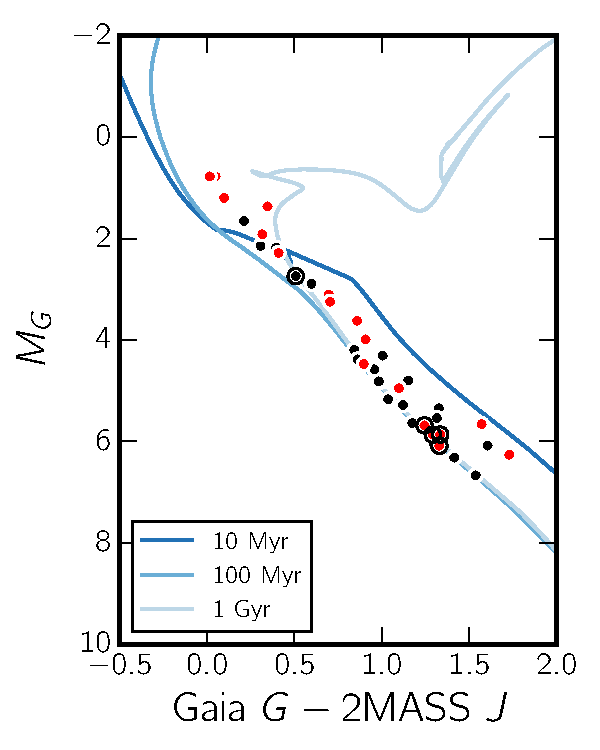
\includegraphics[width=0.7\linewidth]{cmd_gjg.pdf}
  \caption{Color-magnitude diagram of member stars.
    For comparison, we show the MIST isochrones of a solar metallicity population \todo{cite mist}.
    Red markers indicate infrared excess,
    and markers wrapped in black circles indicate X-ray source (Table~\todo{tablenum}).
  }
  \label{fig:cmd_gjg}
\end{figure}
\end{document}
